% !TEX root = ../dw-oefeningen.tex
\documentclass[../dw-oefeningen.tex]{subfiles}
\begin{document}
\chapter{Eenvoudige principes van discrete wiskunde}

\section*{Theorie}

\subsubsection*{2.3.3 Injecties tellen}
Op hoeveel manieren kan ik 6 studenten uit de klas kiezen en in een
rij tegen het bord zetten?

\[ \frac{n!}{(n - 6)!} \]
\(n\): aantal studenten in de klas

\section*{Oefeningen}

\begin{enumerate}
  % Oefening 1
  \item Toon aan: in elke groep van 13 personen zijn er zeker 2 die in dezelfde maand verjaren.
  \\
  12 personen kunnen in 12 verschillende maanden verjaren. De dertiende persoon deelt de
  maand van zijn/haar verjaardag dus met één van de andere personen.
  
  % Oefening 2
  \item Toon aan dat in een groep mensen altijd zeker 2 mensen hetzelfde aantal vrienden in die groep hebben.
  
  % Oefening 3
  \item Een geblinddoekte man heeft een hoop sokken: 10 bruine en 10 grijze.
        Hoeveel moet hij er nemen om zeker een passend paar te hebben?
        Hoeveel moet hij er nemen om zeker een grijs paar te hebben?
        \begin{itemize}
          \item een passend paar: 3
                \begin{enumerate}
                  \item kleur 1
                  \item kleur 1 - klaar
                \end{enumerate}
                \begin{enumerate}
                  \item kleur 1
                  \item kleur 2
                  \item kleur 1 of kleur 2 - klaar 
                \end{enumerate}
        \end{itemize}
  
  % Oefening 4
  \item Stel dat we vijf punten kiezen in een gelijkzijdige driehoek met zijde
        1. Toon aan dat er minstens één paar punten is waarvan de onderlinge
        afstand ten hoogste 1/2 is.
        
        Drie van de punten kunnen in de hoeken van de driehoek liggen. Rond die drie 
        punten trekken we een cirkel met straal 1/2. Het vierde punt kan in het midden
        van de driehoek, buiten de cirkels, liggen. Het vijfde punt ligt ofwel buiten
        de cirkels, en ligt dan op afstand ten hoogste 1/2 van het vierde punt, ofwel
        ligt het binnen één van de cirkels, en dus op afstand ten hoogste 1/2 van het
        middelpunt van die cirkel.
        
        Ofwel: driehoek verdelen in 4 kleinere driehoeken met zijde 1/2. In minstens 
        één driehoek liggen minstens 2 punten.

  % Oefening 5
  \item Toon aan: in elke verzameling van 12 gehele getallen zitten er altijd
        2 waarvan het verschil deelbaar is door 11.
        \begin{align*}
          23 - 1 &= 22      & 22/11 = 2 \\
           23/11 &= 2 + 1   & \\
            1/11 &= 0 + 1   
        \end{align*}

        Getallen waarvan het verschil deelbaar is door 11, hebben dus een
        gelijke rest bij deling door 11.

        Er zijn 11 mogelijke resten bij deling door 11: 0 tot en met 10. We kunnen
        11 getallen hebben met verschillende resten. Het twaalfde getal zal dezelfde
        rest hebben als één van de andere. Het verschil van beide is dus
        deelbaar door 11.
        \begin{align*}
          \exists i \neq j: & a_i = q_i \cdot 11 + r_i \quad (0 \leq r_i \leq 10) \\
                            & a_j = q_j \cdot 11 + r_j \quad (0 \leq r_j \leq 10) \\
                            &\text{ met } r_i = r_j \\
          a_i - a_j &= (q_i \cdot 11 + \cancel{r_i}) - (q_j \cdot 11 + \cancel{r_j}) \\
                    &= (q_i \cdot 11) - (q_j \cdot 11) \\
                    &= (q_i - q_j) \cdot 11 \\
        \end{align*}
        Dus, \(a_i - a_j\) is deelbaar door 11.

\end{enumerate}

\begin{enumerate}[start=10]
  % Oefening 10 
  \item Als je 500000 \enquote{woorden} hebt van 4 of minder letters, kan het dan
        dat ze allemaal verschillend zijn?
        \begin{align*}
          \begin{array}{lrr}
            1 \text{ letter}  & 26^1 = & 26 \\
            2 \text{ letters} & 26^2 = & 676 \\
            3 \text{ letters} & 26^3 = & \num{17576} \\
            4 \text{ letters} & 26^4 = & \num{456976} \\
            \cline{3-3}
                              &        & \num{475254}
          \end{array}
        \end{align*}
        Neen. In totaal zijn er \num{475254} mogelijke woorden, minder dan \num{500000}.
  
\end{enumerate}

\begin{enumerate}[start=16]
  % Oefening 16
  \item In een gemengde groep zitten 32 jongens. Elk van de jongens kent 5
        meisjes van de klas, en elk meisje kent 8 jongens van de klas. Hoeveel
        meisjes zitten er in de klas?
        \begin{align*}
          &|J| = 32, |M| = x \\
          &S = \{(j, m) \in J \times M \mid j \text{ en } m \text{ kennen mekaar}\} \\
          &\forall j \in J: k_j = 5 \\
          &\forall m \in M: r_m = 8 \\
          |S| &= \sum_{j \in J} k_j = \sum_{j \in J} 5 = 32 \cdot 5 \\
              &= \sum_{m \in M} r_m = \sum_{m \in M} 8 = 8 \cdot x \\
        \end{align*}
        \begin{align*}
          8 \cdot x &= 32 \cdot 5 \\
          x &= \frac{32 \cdot 5}{8} \\
          x &= 20
        \end{align*}

\end{enumerate}

\begin{enumerate}[start=20]
  % Oefening 20
  \item Hoeveel woorden van 4 letters uit een alfabet van 10 letters kan je
        maken als elke letter hoogstens 1 keer mag gebruikt worden?
        \\[1em]
        \(\dfrac{n!}{(n-k)!} = \dfrac{10!}{(10-4)!} = \dfrac{10!}{6!} = 10 \cdot 9 \cdot 8 \cdot 7 = \num{5040}\)

\end{enumerate}

\begin{enumerate}[start=23]
  \item Een dominoblokje kan voorgesteld worden als \([x \mid y]\), met \(x, y \in [0..6]\). Toon aan dat er 28 blokjes zijn (en geen 49).
        \[\binom{7+2-1}{2} = \frac{8!}{2!6!} = \frac{8 \cdot 7}{2} = 28\]
\end{enumerate}

\begin{enumerate}[start=25]
  \item Er zitten \(m\) meisjes en \(n\) jongens in een klas. Op hoeveel manieren
        kan je ze in een rij zetten als alle meisjes samen moeten staan?
        \\[1em]
        De meisjes onderling kunnen op \(m!\) manieren geordend worden:
        \[m!\]
        De meisjes kunnen helemaal links, helemaal rechts, of ergens daartussen gezet worden.
        Er zijn dus \(n + 1\) mogelijke plaatsen om de meisjes te zetten:
        \[m!(n + 1)\]
        Op de resterende posities kunnen de jongens op \(n!\) manieren gezet worden:
        \[m!(n + 1)n!\]

\end{enumerate}

\begin{enumerate}[start=35]
  % Oefening 35
  \item Toon aan: als 3 identieke dobbelstenen geworpen worden, zijn er 56
        mogelijke uitkomsten. Hoeveel zijn er bij n identieke dobbelstenen?
      \begin{enumerate}
        \item \(\displaystyle \binom{6 + 3 - 1}{3} = \binom{8}{3} = \frac{8!}{3!5!} = \frac{8 \cdot 7 \cdot 6 \cdot \cancel{5!}}{3!\cancel{5!}} = \frac{8 \cdot 7 \cdot \cancel{6}}{\cancel{3!}} = 56\)
        \item \(\displaystyle \binom{6 + n - 1}{n}\)
      \end{enumerate}

\end{enumerate}

\begin{enumerate}[start=44]
  % Oefening 44
  \item In een klas van 67 wiskundestudenten zijn er 47 die Frans kennen, 35
        die Duits kennen en 23 die zowel Frans als Duits kennen. Hoeveel kennen 
        er geen van beide? Als bovendien 20 studenten Russisch kennen,
        van wie 12 ook Frans en 11 ook Duits kennen en 5 studenten kennen
        de drie talen, hoeveel zijn er dan die geen van de drie kennen?
        \begin{align*}
          |W| = 67 \quad &|F| = 47 \quad |D| = 35 \quad |F \cap D| = 23 \\
        \end{align*}
        \begin{align*}
          |W \setminus (F \cup D)| &= |W| - |F \cup D| \\
                                   &= |W| - (|F| + |D| - |F \cap D|) \\
                                   &= |W| - |F| - |D| + |F \cap D| \\
                                   &= 67 - 47 - 35 + 23 \\
                                   &= 8 \\
        \end{align*}
        \begin{align*}
          |W| = 67 \quad &|F| = 47 \quad |D| = 35 \quad |F \cap D| = 23 \\
                         &|R| =  20 \quad |F \cap R| = 12 \quad |D \cap R| = 11 \quad |F \cap D \cap R| = 5 \\
        \end{align*}
        \begin{align*}
          |W \setminus (F \cup D \cup R)| &= |W| - |F \cup D \cup R| \\
                                        &= |W| - (|F| + |D| + |R| \\
                                        &\quad\quad\quad\quad\quad - |F \cap D| - |F \cap R| - |D \cap R| \\
                                        &\quad\quad\quad\quad\quad + |F \cap D \cap R|) \\
                                        &= 67 - 47 - 35 - 20 + 23 + 12 + 11 - 5 \\
                                        &= 6 \\
        \end{align*}

  % Oefening 45
  \item Hoeveel woorden kan je maken met de letters A, E, M, O, U, Y
        (elk 1 keer gebruiken) als de opeenvolgingen ME en YOU niet mogen
        voorkomen?
        \begin{align*}
                W &= \text{alle woorden met de 6 letters} \\
           W_{ME} &=  \text{alle woorden waar ME in voorkomt} \\
          W_{YOU} &=  \text{alle woorden waar YOU in voorkomt}
        \end{align*}
        \begin{align*}
          |W \setminus (W_{ME} \cup W_{YOU})| &= |W| - (|W_{ME}| + |W_{YOU}| - (|W_{ME} \cap W_{YOU}|)) \\
          &\quad\text{met}\quad
          \begin{alignedat}{2}
            |W| &= 6! &&= 720
          \end{alignedat}
          \\[1em]
          \intertext{Er zijn 5 plaatsen waar de M gezet kan worden. Niet op de laatste plaats, 
                     want er moet nog plek zijn voor de E. De overige 4 letters kunnen op \(4!\) manieren gezet worden.}
          &\quad\quad
          \begin{alignedat}{2}
            |W_{ME}| &= 5 \cdot 4! = 5! \\
          \end{alignedat} 
          \\[1em]
          \intertext{Er zijn 4 plaatsen waar de Y gezet kan worden. Niet op de laatste twee plaatsen, 
                     want er moet nog plek zijn voor de OU. De overige 4 letters kunnen op \(3!\) manieren gezet worden.}
          &\quad\quad
          \begin{alignedat}{2}
            |W_{YOU}| &= 4 \cdot 3! = 4!
          \end{alignedat} 
          \\[1em]
          \intertext{Als we ME en YOU, en de resterende letter, als objecten beschouwen, moeten we drie
                     objecten een plaats geven. Dat kan op \(3!\) manieren.}
          &\quad\quad
          \begin{alignedat}{2}
            |W_{ME} \cap W_{YOU}| &= 3!
          \end{alignedat}
          \\[1em]
          &= 720 - (5! + 4! - 3!) \\
          &= 720 - (120 + 24 - 6) \\
          &= 720 - 138 \\
          &= 582
        \end{align*}
\end{enumerate}

\section*{Examen 2018}

\begin{enumerate}
  \item In de volgende opgaven wordt gevraagd om woorden te tellen. Een \emph{woord} is voor ons
        eenvoudigweg een opeenvolging van een aantal letters: we beperken ons hier dus niet 
        tot wat we in het woordenboek terugvinden! Een uitdrukking met sommen, verschillen en
        producten van getallen (en eventueel binomiaalcoëfficiënten) volstaat telkens als antwoord.
        Je hoeft de resultaten dus niet per se volledig uit te rekenen.
        
        \begin{enumerate}
          \item Hoeveel woorden van van zeven letters kun je maken met de letters a, b, c en d (bv.
                \emph{caaddac} of \emph{bbbbbbb})?
                \\[1em]
                7 keer kiezen uit 4 letters, volgorde is van belang:
                \[4^7\]

          \item In hoeveel van deze woorden komt de letter d minstens één keer voor?
                \\[1em]
                Totaal aantal woorden - aantal woorden zonder d:
                \[4^7 - 3^7\]

          \item In hoeveel van deze woorden komt de letter a precies drie keer voor?
                \\[1em]
                We moeten drie keer een positie kiezen om een a te zetten. We kunnen niet drie keer dezelfde
                positie kiezen, want dan hebben we maar één a. Herhaling is dus niet toegestaan.
                \[\binom{7}{3} = \frac{7!}{3!(7-3)!} = \frac{7!}{3!4!} = \frac{7 \cdot \cancel{6} \cdot 5 \cdot \cancel{4!}}{\cancel{3!}\cancel{4!}} = 35\]
                Er zijn \(3^4\) manieren om de overige \(4\) letters te kiezen uit de resterende \(3\) letters.
                \[35 \cdot 3^4\]


          \item In hoeveel van deze woorden komt elk van de letters a, b, c en d minstens één keer
                voor (bv. \emph{aacddbb}, maar niet \emph{cadacad})?
                \begin{align*}
                  W &= 4^7 \\
                  W_{\cancel{a}} = W_{\cancel{b}} = W_{\cancel{c}} = W_{\cancel{d}} &= 3^7 \\
                \end{align*}
                \begin{align*}
                  &|W \setminus (W_{\cancel{a}} \cup W_{\cancel{b}} \cup W_{\cancel{c}} \cup W_{\cancel{d}})|\\
                  &= |W| - |W_{\cancel{a}} \cup W_{\cancel{b}} \cup W_{\cancel{c}} \cup W_{\cancel{d}}| \\
                  %%%%%
                  &= |W| - ( \\
                  &\qquad |W_{\cancel{a}}| + |W_{\cancel{b}}| + |W_{\cancel{c}}| + |W_{\cancel{d}}| \\
                  &\qquad - (|W_{\cancel{a}} \cap W_{\cancel{b}}| + |W_{\cancel{a}} \cap W_{\cancel{c}}| + |W_{\cancel{a}} \cap W_{\cancel{d}}| + |W_{\cancel{b}} \cap W_{\cancel{c}}| + |W_{\cancel{b}} \cap W_{\cancel{d}}| + |W_{\cancel{c}} \cap W_{\cancel{d}}|)  \\
                  &\qquad + (|W_{\cancel{a}} \cap W_{\cancel{b}} \cap W_{\cancel{c}}| + |W_{\cancel{a}} \cap W_{\cancel{b}} \cap W_{\cancel{d}}| + |W_{\cancel{a}} \cap W_{\cancel{c}} \cap W_{\cancel{d}}| + |W_{\cancel{b}} \cap W_{\cancel{c}} \cap W_{\cancel{d}}|) \\
                  &\qquad - |W_{\cancel{a}} \cap W_{\cancel{b}} \cap W_{\cancel{c}} \cap W_{\cancel{d}}| \\
                  &\qquad) \\
                  %%%%%
                  &= 4^7 - ( \\
                  &\qquad 3^7 + 3^7 + 3^7 + 3^7 \\
                  &\qquad - (2^7 + 2^7 + 2^7 + 2^7 + 2^7 + 2^7) \qquad \text{(enkel de resterende 2 letters gebruiken)} \\
                  &\qquad + (1^7 + 1^7 + 1^7 + 1^7) \qquad \text{(slechts één letter gebruiken)} \\
                  &\qquad - 0 \qquad \text{(geen enkele letter gebruiken: kan niet)} \\
                  &\qquad) \\
                  %%%%%
                  &= 4^7 - (4 \cdot 3^7 - 6 \cdot 2^7 + 4 \cdot 1^7 - 0) \\
                \end{align*}

          \item Hoeveel woorden van vijf letters kun je maken met de letters a, b, c en d als twee
                van deze letters precies twee keer dienen voor te komen (bv. \emph{accad} of \emph{bddcc}, maar
                niet \emph{bbbaa} of \emph{aabcd})?
        \end{enumerate}
\end{enumerate}

\section*{Examen ????}
Op hoeveel manieren kunnen we op het onderstaande \enquote{schaakbord} (met 40 zwarte en 40 witte vakken)
pionnen plaatsen ...
\begin{enumerate}
  \item vier identieke pionnen plaatsen op verschillende vakken?
  \item vier identieke pionnen plaatsen op verschillende vakken als deze niet alle van dezelfde kleur mogen zijn?
  \item vier identieke pionnen plaatsen op verschillende vakken die niet alle in dezelfde rij liggen, en niet alle van dezelfde kleur zijn?
  \item vier identieke pionnen plaatsen op niet noodzakelijk verschillende vakken als de pionnen niet alle in dezelfde kolom mogen liggen?
\end{enumerate}

\noindent\textbf{N.B.} We houden hierbij geen rekening met welke pion als eerste wordt geplaatst,
welke als tweede, enz. Een uitdrukking met sommen, verschillen en producten van getallen
(en eventueel binomiaalcoëfficiënten) volstaat telkens als antwoord. De resultaten hoeven
dus niet per se volledig te worden uitgerekend.

\begin{figure}[H]
  \centering

  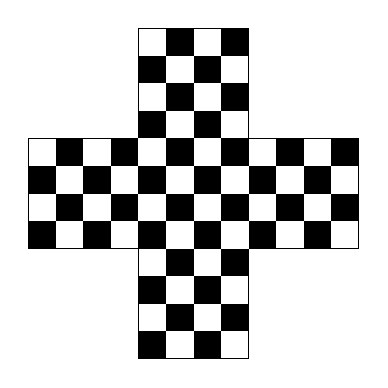
\begin{tikzpicture}[scale=0.35]
    % Horizontale lijnen
    \draw (4,12) -- (8,12);
    \draw (0, 8) -- (4, 8);
    \draw (8, 8) -- (12,8);
    \draw (0, 4) -- (4, 4);
    \draw (8, 4) -- (12,4);
    \draw (4, 0) -- (8, 0);

    % Verticale lijnen
    \draw (0, 4) -- (0, 8);
    \draw (4, 8) -- (4,12);
    \draw (4, 0) -- (4, 4);
    \draw (8, 8) -- (8,12);
    \draw (8, 0) -- (8, 4);
    \draw (12,4) -- (12,8);


    % teken het kruis: alle (x,y) met x in 4..7 of y in 4..7, 0<=x,y<=11
    \foreach \x in {0,...,11} {
      \foreach \y in {0,...,11} {
        \pgfmathtruncatemacro{\inC}{(\x>=4 && \x<=7) || (\y>=4 && \y<=7)}
        \ifnum\inC=1\relax
          \pgfmathtruncatemacro{\p}{mod(\x+\y,2)}
          \ifnum\p=0\relax
            \fill[black] (\x,\y) rectangle ++(1,1);
          \fi
          % \draw (\x,\y) rectangle ++(1,1);
        \fi
      }
    }
  \end{tikzpicture}
\end{figure}

\begin{enumerate}
  \item Dit komt neer op 4 vakken kiezen:
        \[\binom{80}{4} = \frac{80!}{(80-4)!4!}\]

  \item Kies een wit vak, kies een zwart vak, en kies de laatste twee uit de resterende 78 vakken:
        
        \begin{align*}
            \binom{40}{1} \cdot \binom{40}{1} \cdot \binom{78}{2} 
            &= 40 \cdot 40 \cdot \frac{78!}{76!2!} \\
            &= 1600 \cdot \frac{78 \cdot 77}{2} \\
            &= 1600 \cdot 39 \cdot 77 \\
            &= \num{1238400} 
        \end{align*}

        Ofwel: totaal - allemaal wit - allemaal zwart:
        \begin{align*}
          \binom{80}{4} - \binom{40}{4} - \binom{40}{4} 
          &= \frac{80!}{76!4!} - \frac{40!}{36!4!} - \frac{40!}{36!4!} \\
          &= \frac{80!}{76!4!} - 2 \cdot \frac{40!}{36!4!} \\
          &= \frac{80 \cdot 79 \cdot 78 \cdot 77}{4!} - 2 \cdot \frac{40 \cdot 39 \cdot 38 \cdot 37}{4!} \\
          &= \frac{80 \cdot 79 \cdot 78 \cdot 77 - 2 \cdot 40 \cdot 39 \cdot 38 \cdot 37}{4!} \\
          &= \frac{80 \cdot 79 \cdot 78 \cdot 77 - 2 \cdot 40 \cdot 39 \cdot 38 \cdot 37}{24} \\
          &= \num{1238400}
        \end{align*}

  \item Eerst twee rijen kiezen en daarin een vak kiezen, is moeilijk aangezien er rijen zijn met 
        4 vakken en rijen met 12 vakken. Beter dus met inclusie/exclusie werken:
        \\
        totaal - (allemaal zelfde kleur (K) + allemaal zelfde rij (R()))
        \begin{align*}
          \binom{80}{4} - ( |K| \cup |R| )
          &= \binom{80}{4} - ( |K| + |R| - |K \cap R| ) \\
          &= \binom{80}{4} - \left( 
            2 \cdot \binom{40}{4} 
            + \left(
                8 \cdot \binom{4}{4} 
                + 4 \cdot \binom{12}{4}
              \right)
            - \left(4 \cdot 2 \cdot \binom{6}{4} \right)
          \right) \\
        \end{align*}

  \item Nu is wel herhaling toegestaan.
        totaal - allemaal zelfde kolom (K)
        \begin{align*}
          &\binom{80 + 4 - 1}{4} - \left(
            8 \cdot \binom{4 + 4 - 1}{4} + 4 \cdot \binom{12 + 4 - 1}{4}
          \right) \\
          &= \frac{83!}{4!(83-4)!} - \left(
            8 \cdot \frac{7!}{4!(7-4)!} + 4 \cdot \frac{15!}{4!(15-4)!}
          \right)
        \end{align*}
\end{enumerate}

\section*{Samenvatting}
\noindent
Gegeven: \(|A| = k \quad |B| = n\)
\\
H: herhaling toegestaan \\
V: volgorde maakt uit
\begin{align*}
                                         \# f : A \to B &= n^k                                       \quad &\text{H \quad V}\\
           (k \leq n) \# \text{ injecties } f : A \to B &= \frac{n!}{(n-k)!}                         \quad &\text{\cancel{H} \quad V} \\
              (k = n) \# \text{ bijecties } f : A \to B &= n! \\
              (k \leq n) \# k-\text{deelverzamelingen van } B &= \binom{n}{k} = \frac{n!}{k!(n-k)!} \quad &\text{\cancel{H} \quad \cancel{V}} \\
              \# \text{ herhalingscombinaties v } k \text{ uit } n &= \binom{n+k-1}{k}               \quad &\text{H \quad \cancel{V}}\\
  \\[1em]
  \quad
  \begin{rcases}
    |\text{Im}(f)| = k = n = |B| \\
    \text{Im}(f) \subset B
  \end{rcases} &\Rightarrow \text{Im}(f) = B \\
\end{align*}

\begin{align*}
  | A \cup B | &= |A| + |B| - | A \cap B | \\
  | A \cup B \cup C | &= |A| + |B| + |C|  \\
                      &- | A \cap B | - | A \cap C | - | B \cap C | \\
                      &+ | A \cap B \cap C | \\
  | A \cup B \cup C \cup D | &= |A| + |B| + |C| + |D| \\
                             &- | A \cap B | - | A \cap C | - | A \cap D | - | B \cap C | - | B \cap D | - | C \cap D | \\
                             &+ | A \cap B \cap C | + | A \cap B \cap D | + | A \cap C \cap D | + | B \cap C \cap D | \\
                             &- | A \cap B \cap C \cap D | \\
\end{align*}

\end{document}